% !TEX encoding = UTF-8
% !TEX TS-program = pdflatex
% !TEX root = ./tesi.tex

%**************************************************************
\section{Synthetic}\label{sec:synthetic}
%**************************************************************

As in there are few real-life datasets for visual odometry, we decided to create a synthetic dataset by using BlenderProc2 framework,
which is a procedural photo-realistic rendering framework, and it allows to:
\begin{itemize}
    \item \textbf{Loading}: *\textit{.obj}, *\textit{.ply}, *\textit{.blend}, \textit{BOP}, \textit{ShapeNet} etc.
    \item \textbf{Objects}: set or sample objects poses, apply physics and collision checking.
    \item \textbf{Materials}: set or sample physically-based materials and textures.
    \item \textbf{Lighting}: set or sample lights, automatic lighting of 3D-front scenes.
    \item \textbf{Cameras}: set, sample or load camera poses from file.
    \item \textbf{Rendering}: RGB, stereo, depth, normal and segmentation images/sequences.
    \item \textbf{Writing}: *.hdf5 containers, \textit{COCO} and \textit{BOP} annotations.
\end{itemize}

\subsection{Scene}\label{subsec:scene}
To create the synthetic dataset, the first thing is to create a scene with customized objects, material and textures.
\begin{figure}[H]
    \centering
    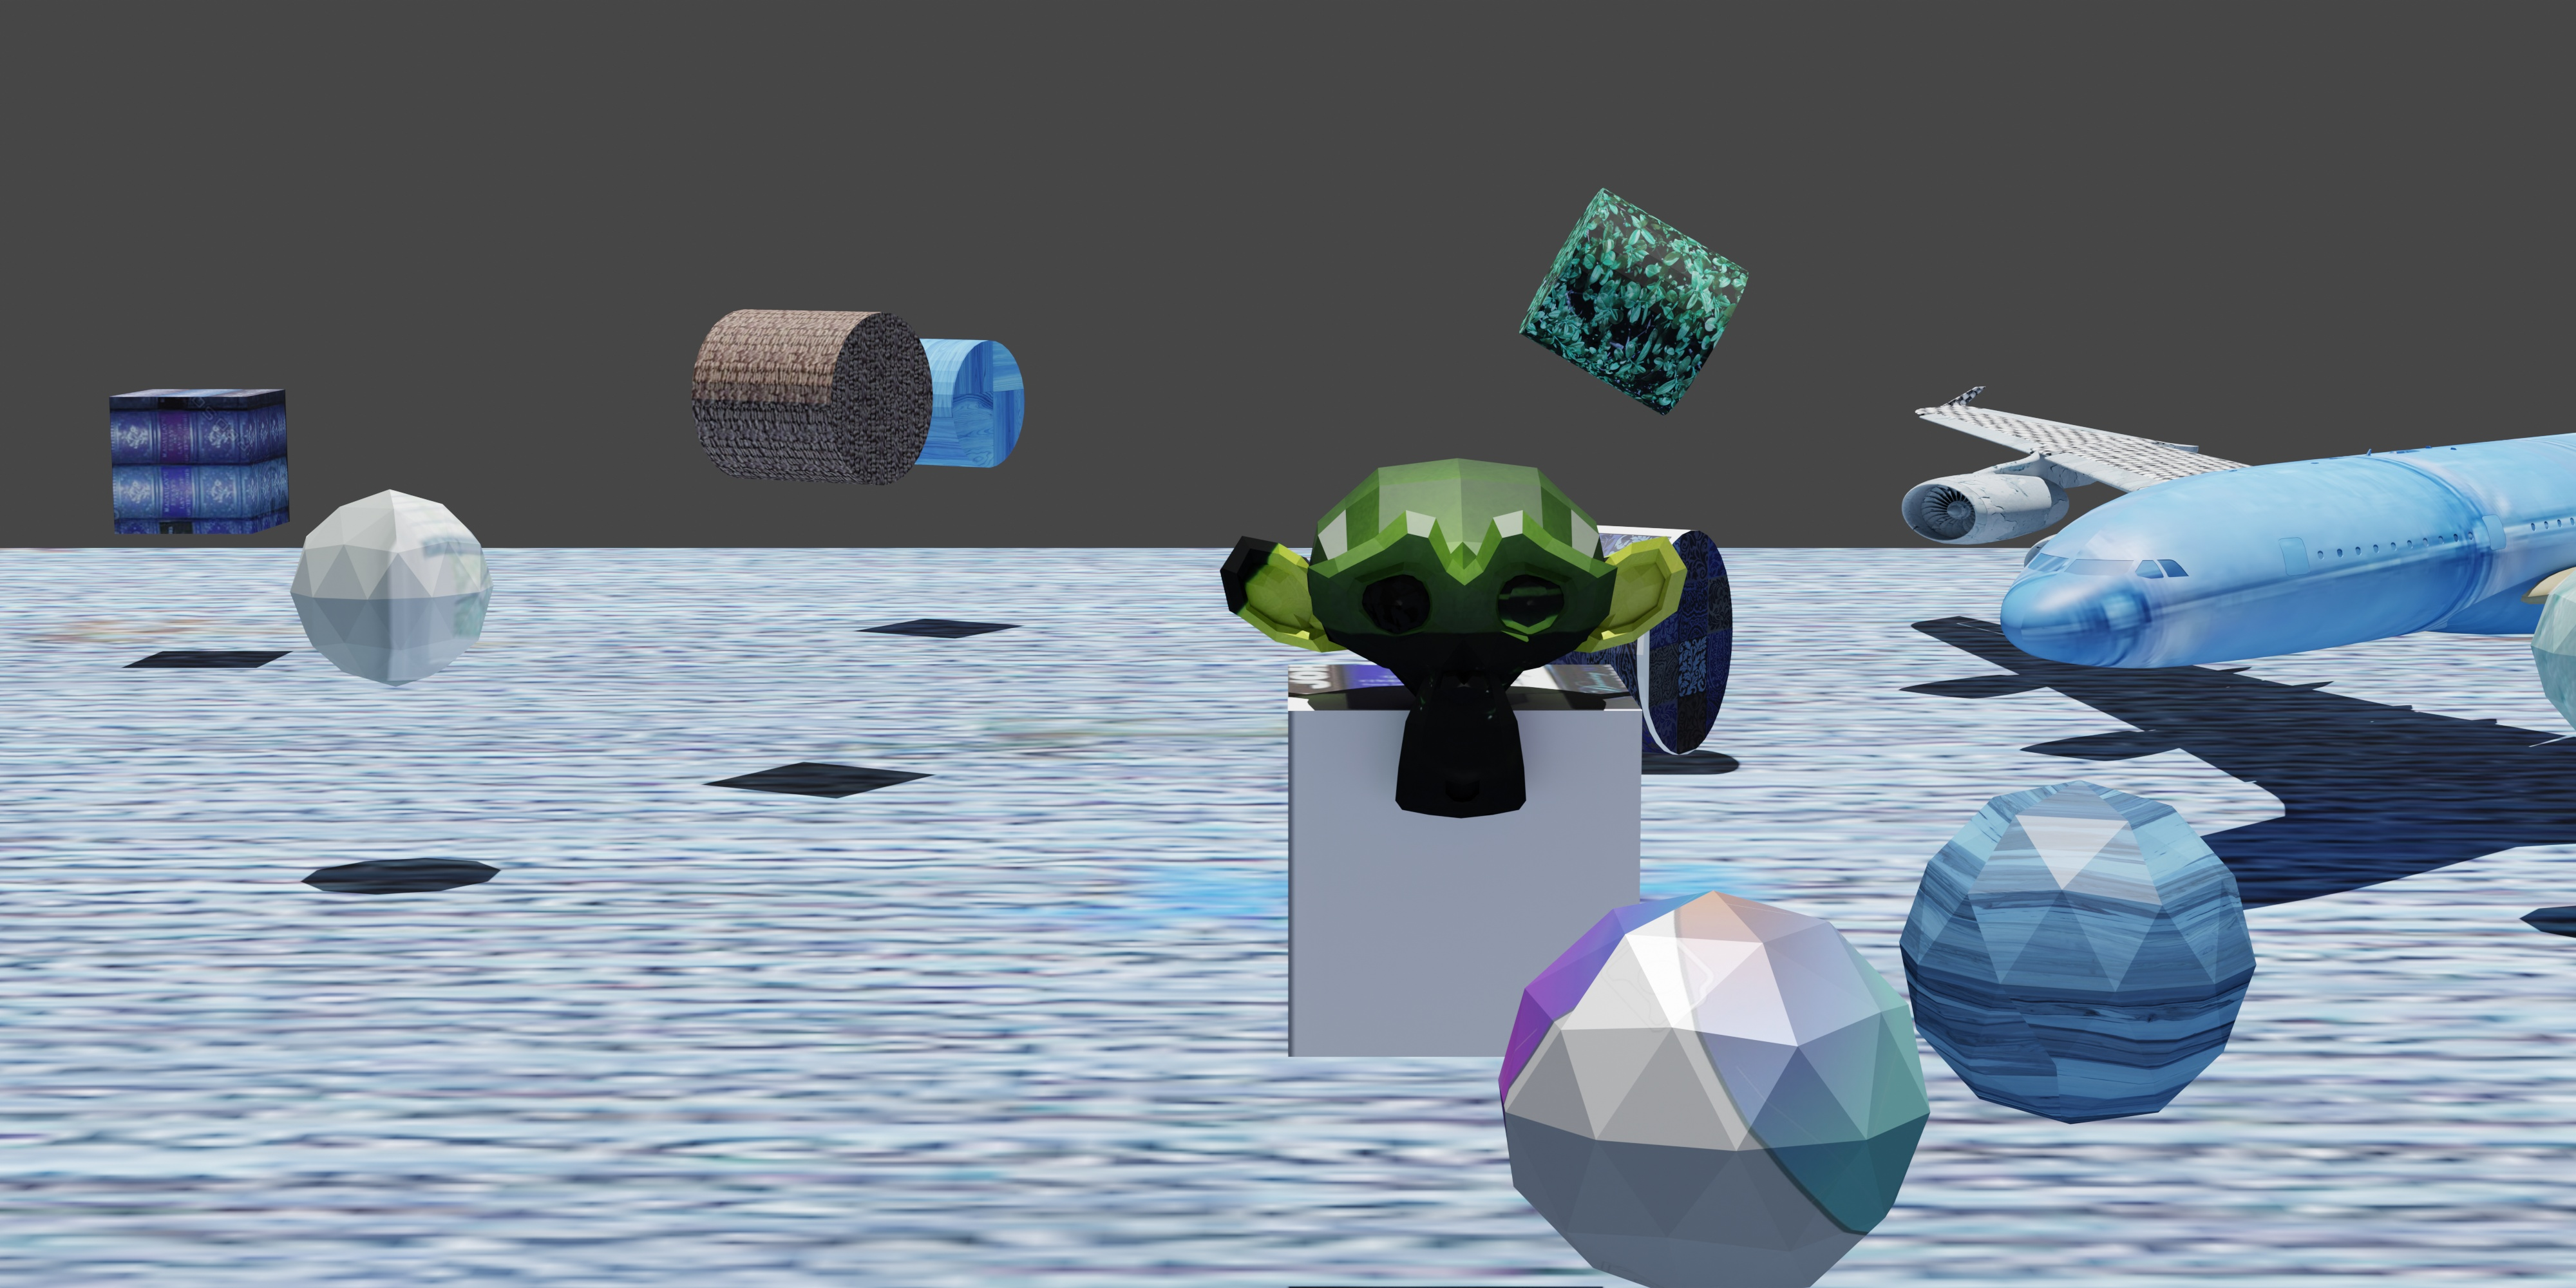
\includegraphics[width=\textwidth]{images/3_example_of_scene}
    \caption{Example of scene}\label{fig:example-of-scene}
\end{figure}
The scene is composed by a set of objects, more precisely:
\begin{itemize}
    \item \textbf{a monkey}: which is at the centre of the scene over a cube.
    \item \textbf{a plane}: which is at left corner of the scene.
    \item \textbf{a set of cubes and spheres}: which are placed randomly in the scene.
\end{itemize}

When rendering the scene, the textures are loaded \textit{randomly}, in the way that in different sequences the textures are different.
\subsection{Image generation}\label{subsec:image-generation}
To generate the sequences, we need to choose the camera position in the scene to do so, we choose randomly a position sampler from the following set for each new pose:

\begin{itemize}
    \item \textbf{disk}: samples a point on a circle or on a 2-ball or on an arc/sector with an inner angle less or equal to 180 degrees.
    \item \textbf{sphere}: samples a point from the surface or from the interior of a solid sphere.
    \item \textbf{part-sphere}: samples a point from the surface or from the interior of a solid sphere which is split in two parts.
    \item \textbf{shell}: samples a point from the volume between two spheres (with radius of the spheres given as parameters).
\end{itemize}
once we have the next position of the camera, we compute the rotation matrix to be applied to the camera in the way that the camera is always looking at the POI (Point Of Interest) which corresponds to the centre of the scene.
\begin{lstlisting}[label={lst:compute-camera-rotation}, caption={Computes the rotatition matrix for the camera.}, captionpos=b]
rotation = bproc.camera.rotation_from_forward_vec(poi - new_position)
\end{lstlisting}
Then, we apply the rotation matrix to the camera and we generate the image, and by setting a certain number of frames between two poses, the framework renders a sequence of images with relative intermediate poses.


But sometime, it happens that the new camera pose is too close to an object of the scene, so we set two conditions that need to be satisfied, otherwise the sampled camera pose is skipped.
The first condition checks if there are obstacles in front of the camera which are too far or too close based on the given \textit{proximity\_checks}, while the second evaluates the interestingness or coverage of the scene.
\begin{lstlisting}[label={lst:lstlisting}, caption={Checks whether the camera pose satisfies the conditions.}, captionpos=b]
def check_pose(c2w_m, special_obj, bvh_tree):
    if not bproc.camera.perform_obstacle_in_view_check(c2w_m, {"min": 5.0}, bvh_tree):
        return False
    if bproc.camera.scene_coverage_score(c2w_m, special_objects=special_obj) < 0.7:
        return False
    return True
\end{lstlisting}


But when the new position is too far away from the old position, the rotation of the camera assumes a wrong value during the transition, because it rotates counter-clockwise instead of clockwise, or vice-versa.
For example:
If we sample the camera position from a disk at 0, 90, 180, 270 degrees, the rotations should be as in the figure 3.1:
\begin{figure}[H]
    \centering
    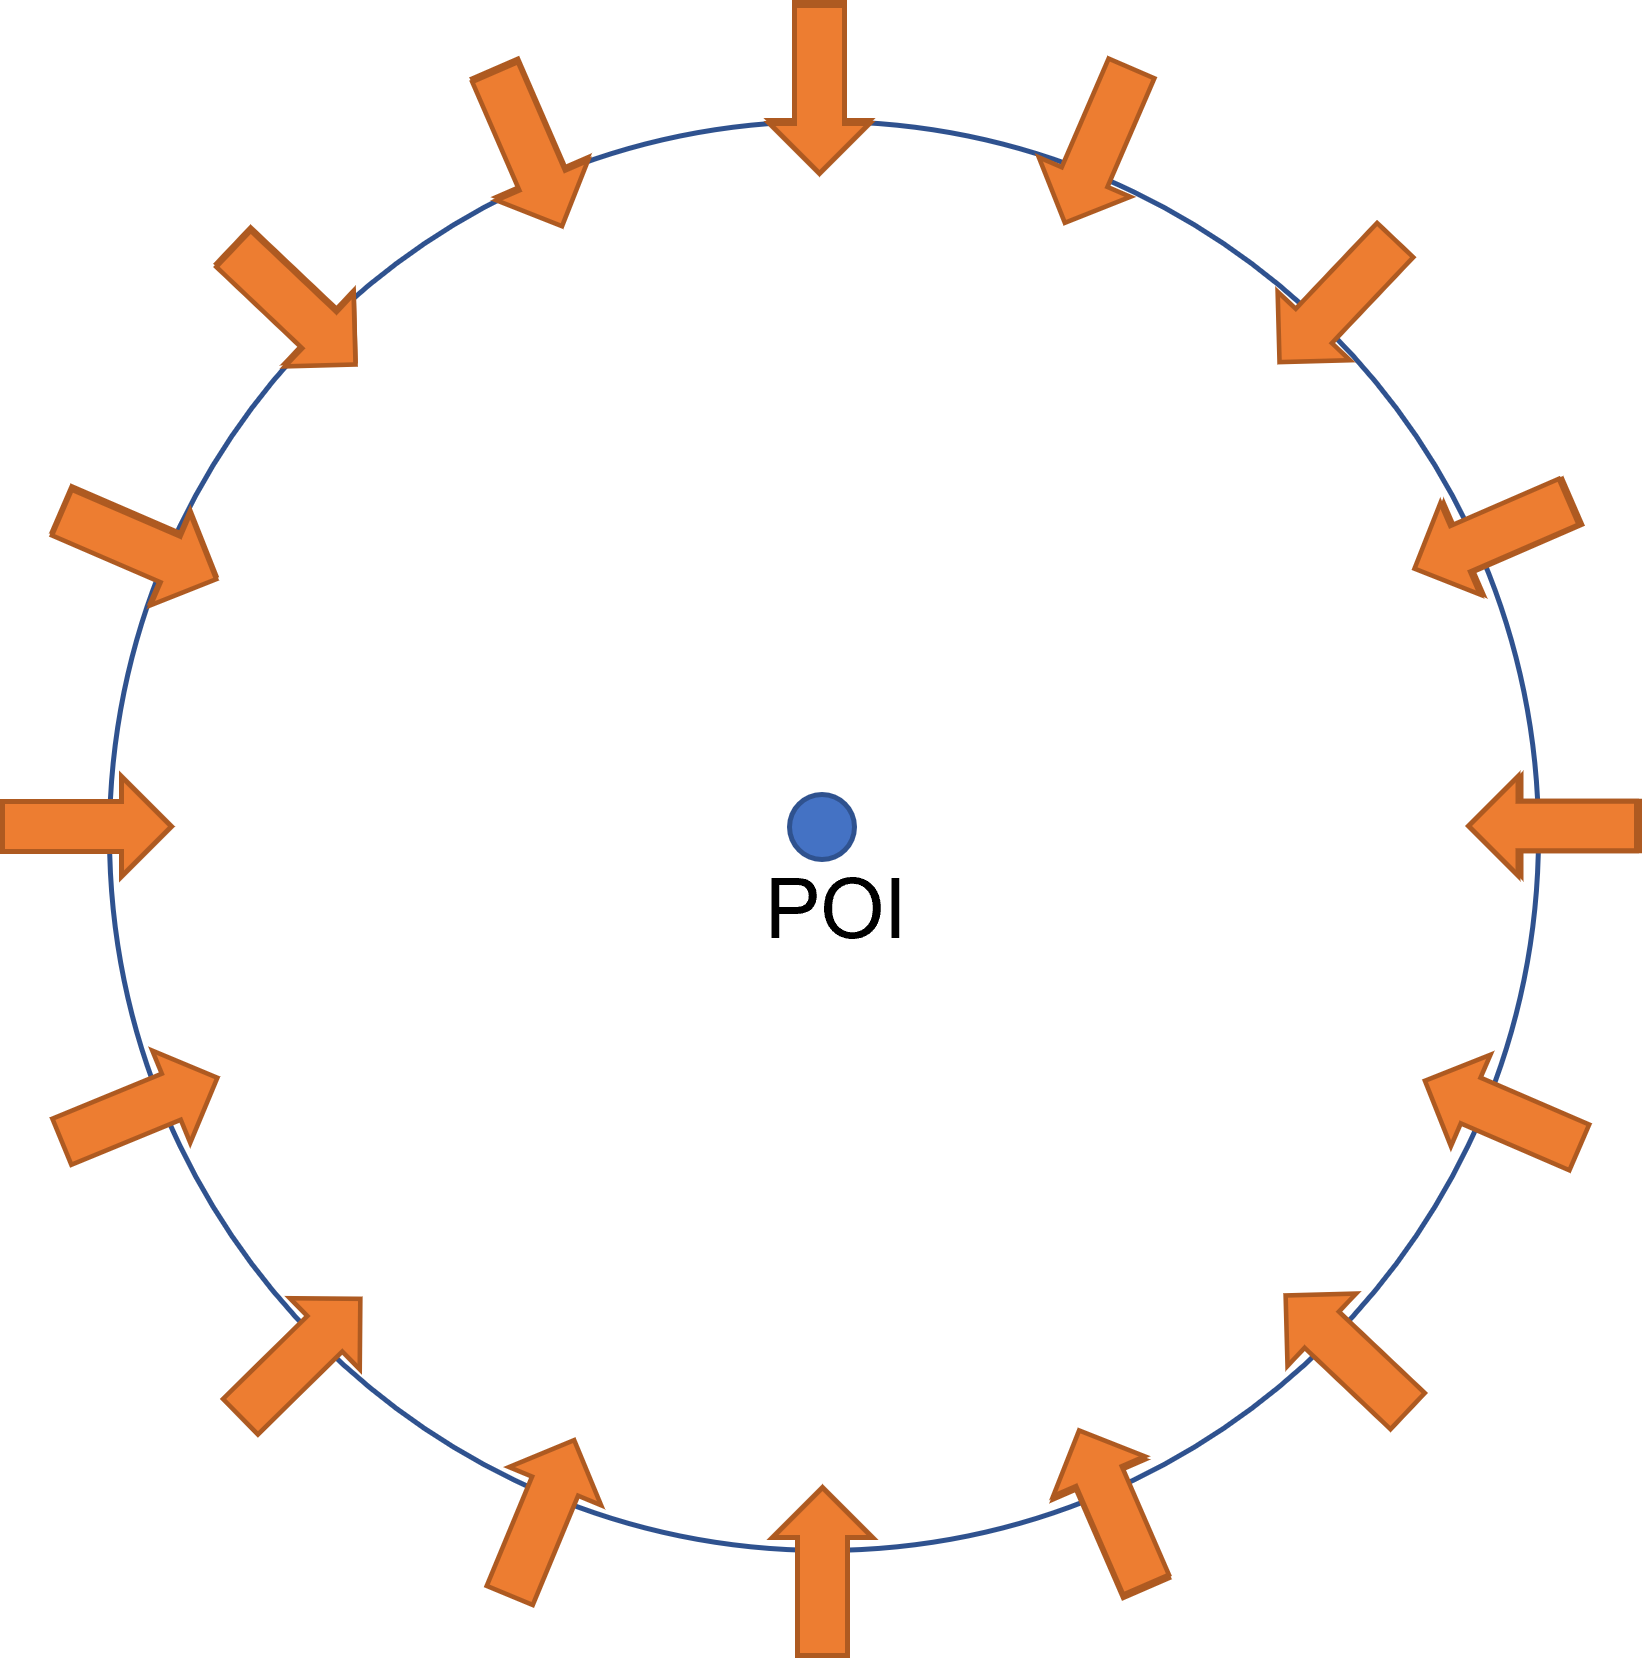
\includegraphics[width=0.5\textwidth]{images/3_correct_transitions}
    \caption{Correct transition on the disk}\label{fig:correct-transition}
\end{figure}

But, the transition from 180 to 270 degrees we obtain is a wrong rotation which is like in figure 3.2:
\begin{figure}[H]
    \centering
    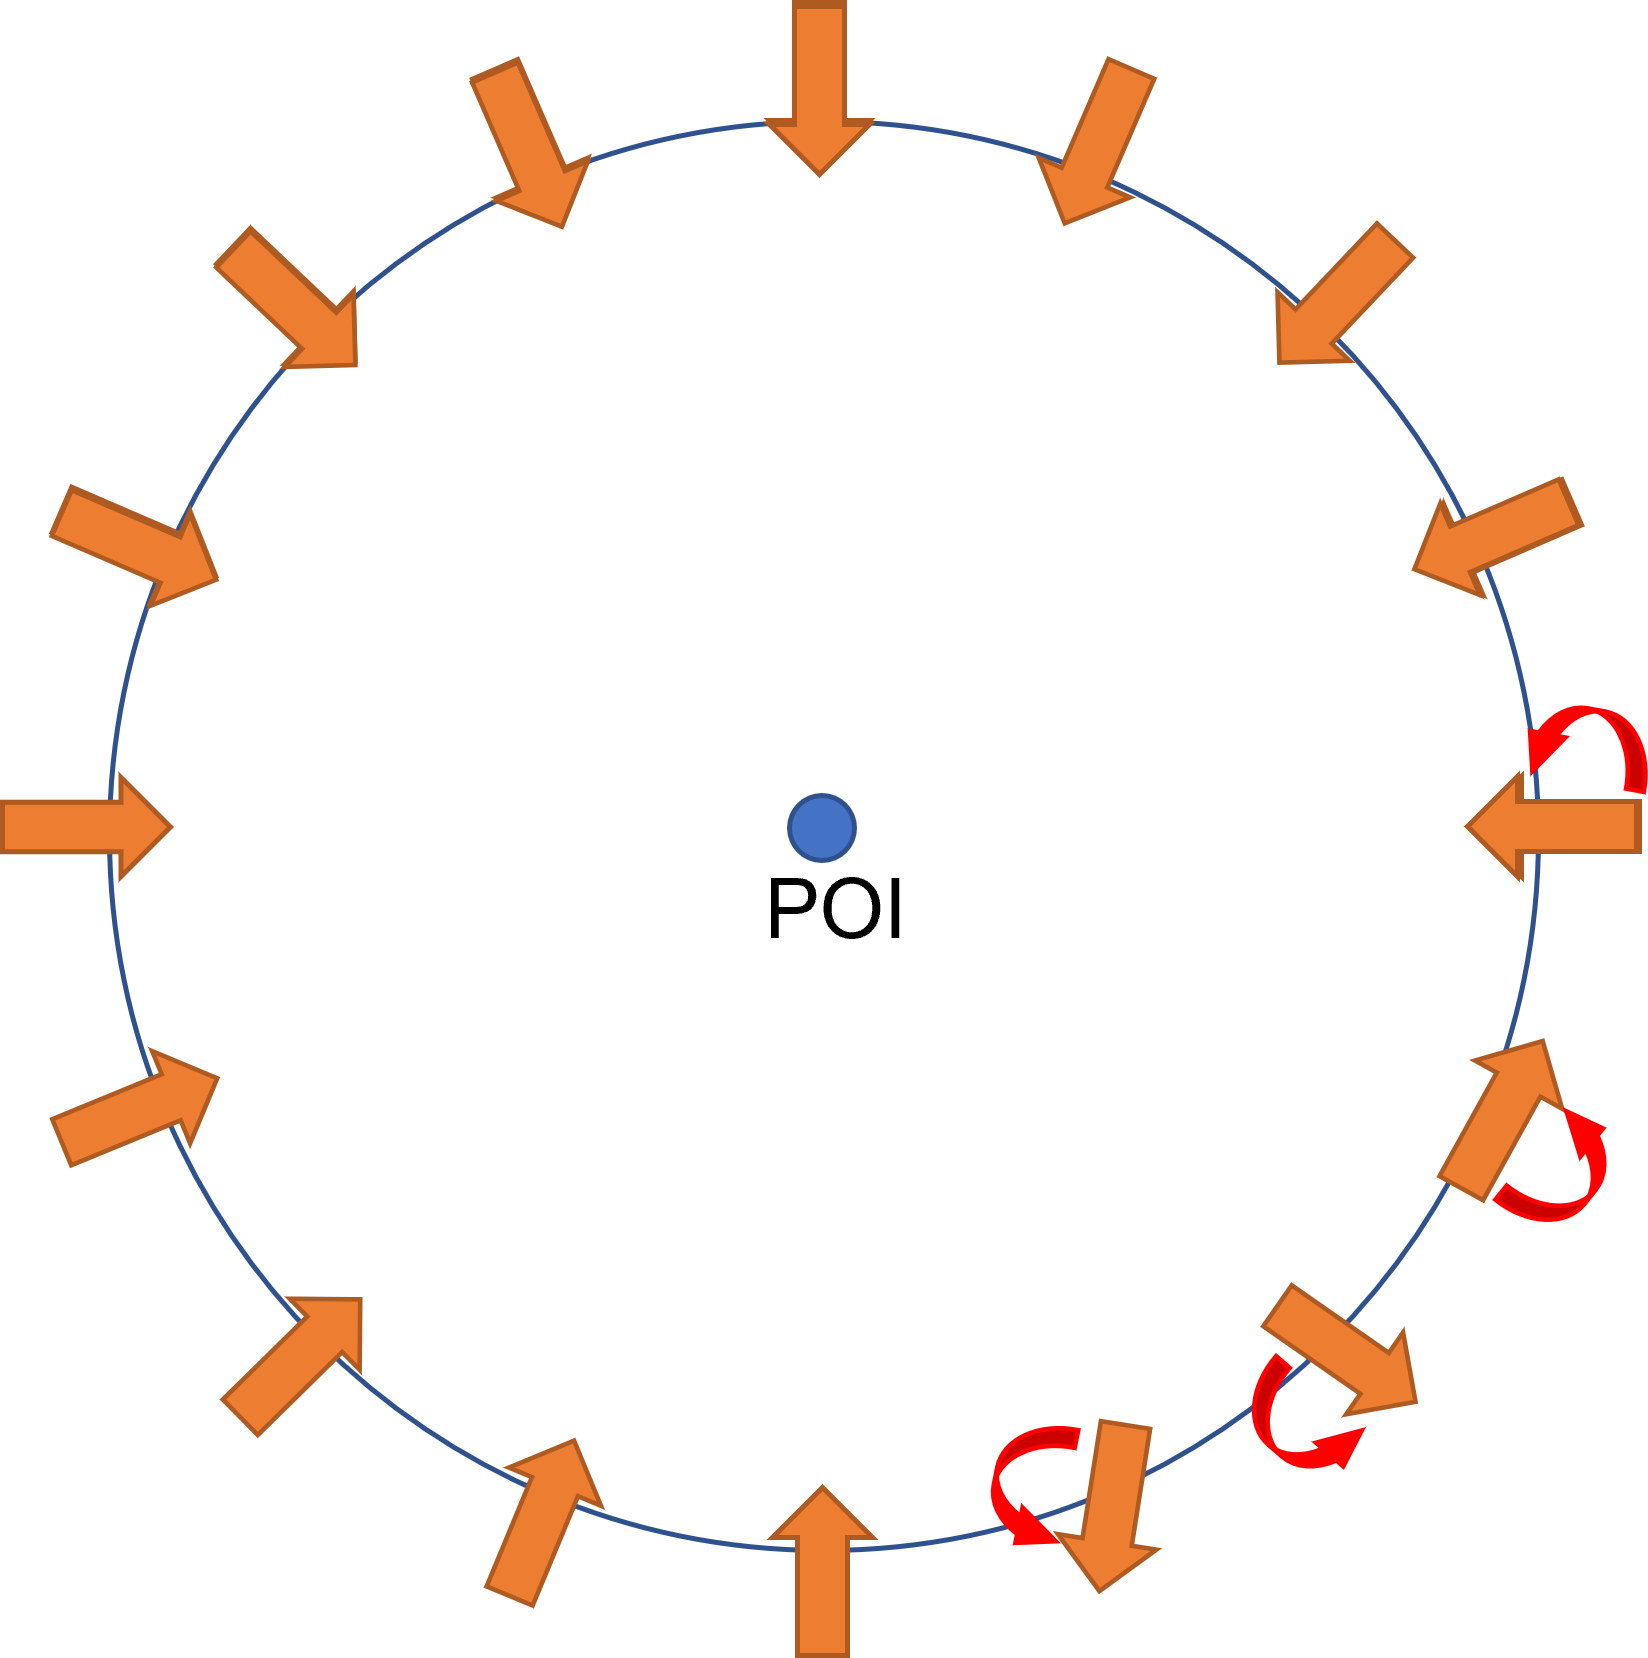
\includegraphics[width=0.5\textwidth]{images/3_wrong_transitions}
    \caption{Wrong transition on the disk}\label{fig:wrong-transition}
\end{figure}

To solve this problem, we tried different solutions: as first, we sample the next pose near to the previous one, but this solution sometime still fails.
The final solution was to sample the new position as previously defined with samplers, but instead of letting the framework to compute the intermediate poses, we manually interpolate them, and by setting frame number to one, we obtain a sequence of correctly rotating images.

\subsection{Dataset statistics}\label{subsec:dataset-statistics}
In total, we have generated 14 sequences, which are divided as follow:
\begin{table}[H]
    \center
    \begin{tabular}{|c|c|c|}
        \hline
        \textbf{Sets}           & \textbf{N. of Sequence} & \textbf{N. Image} \\ \hline
        \textbf{Training set}   & 12                      & 29.100            \\ \hline
        \textbf{Validation set} & 1                       & 1.002             \\ \hline
        \textbf{Test set}       & 1                       & 1.003             \\ \hline
        \textit{\textbf{Total}} & 14                      & 31.105            \\ \hline
    \end{tabular}\caption{Synthetic dataset statistics}
    \label{tab:synthetic-dataset-statistics}
\end{table}
Each image has dimension of 1024x308 pixels with 3 RGB channels.
The whole dateset has dimension \textbf{1.69 GB}.
\subsection{Usage}\label{subsec:usage}
By using the dataset at training time the loss function is highly variable reaching values of \textbf{thousands}, also because the \textbf{Kitti} dataset is much fluid as the trajectory and the camera rotation angles are very small, so, the sequences generated are not similar to the real dataset.